\documentclass{amsart}
\usepackage{hyperref}
\usepackage{minted}
\usepackage{graphicx}

\title{Physically Based Rendering}
\author{Arden Rasmussen}
\date{\today}

\begin{document}
\maketitle

\section{Introduction}%
\label{sec:Introduction}

This paper describes the implementation of a simplistic physically based
renderer TRM\footnote{\url{https://github.com/LuxAter/trm}}. TRM is a minimal
physically based renderer that utilizes ray marching.


\section{Shading}%
\label{sec:Shading}

Currently to simplify the implementation, the renderer only supports three
bidirectional shading functions:
\begin{enumerate}
  \item Specular reflection
  \item Specular transmission
  \item Lambertian diffuse
\end{enumerate}

\subsection{Specular Reflection}%
\label{sub:Specular Reflection}
Specular reflection is the shading for objects that are perfectly reflective,
such as mirrors.

\subsection{Specular Transmission}%
\label{sub:Specular Transmission}
Specular transmission is the shading method for objects that are transmissive,
such as glass or water.

\subsection{Lambertian Diffuse}%
\label{sub:Lambertian Diffuse}
Lambertian diffuse shading is for all other objects, at the moment there are no
material shaders that combine some combination of these three.

\section{SDF}%
\label{sec:sdf}

\subsection{Objects}%
\label{sub:Objects}

There are a number which can be used to construct a scene, and more objects can
easily be added, by simply defining their signed distance functions.

\begin{enumerate}
  \item Sphere
  \item Box
  \item Cylinder
  \item Torus
  \item Plane
  \item Pyramid
  \item MengerSponge
  \item SerpinskiTetrahedron
\end{enumerate}

\subsection{Operations}%
\label{sub:Operations}

There are also a number of operations that can be done to each SDF, which in
turn defined a new SDF. This means that operations can easily be concatenated.

\begin{enumerate}
  \item Elongate
  \item Round
  \item Onion
  \item Union
  \item Subtraction
  \item Intersection
  \item SmoothUnion
  \item SmoothSubtraction
  \item SmoothIntersection
\end{enumerate}

\section{Optimization}%
\label{sec:Optimization}

Optimization is fairly easy to implement by using
OpenMP\footnote{\url{https://www.openmp.org/}}

\begin{minted}[frame=lines,fontsize=\footnotesize]{cpp}
  #pragma omp parallel for schedule(dynamic, 256) shared(buffer)
\end{minted}

This line is placed directly prior to the main render loop. It splits the loop
into chunks of 256 steps, and dynamically allocates the chunks to each of the
available threads. The final part of the line declares that the image buffer is
shared by each thread.

For more information on how OpenMP is used, visit the OpenMP documentation.

\section{Results}%
\label{sec:Results}

Here are some results of the renderer. A serious next step would be to
implement multiple importance sampling. Currently each reflection/transmission
is sampled based on the probability density of the material. In contrast to
that there is light sampling, where the direction of the reflection could be
sampled based upon the direction to light sources.

Each sampling method provides better results based on different materials. For
example material sampling is far superior for very glossy surfaces, such as the
perfect mirror, and light sampling is much better suited for diffuse materials.

Currently TRM does not support light base sampling, which means that scenes
with a large number of diffuse materials take very long to converge to
acceptable results. The best method is to use multiple importance sampling,
which samples the outgoing reflected direction based both on the material and
the light sources.

\begin{figure}[!htb]
  \minipage{0.45\textwidth}
    \includegraphics[width=\linewidth]{figures/objs.png}
    \caption{A showcase of all the possible primitives with the basic material
      types.}
  \endminipage\hfill
  \minipage{0.45\textwidth}
    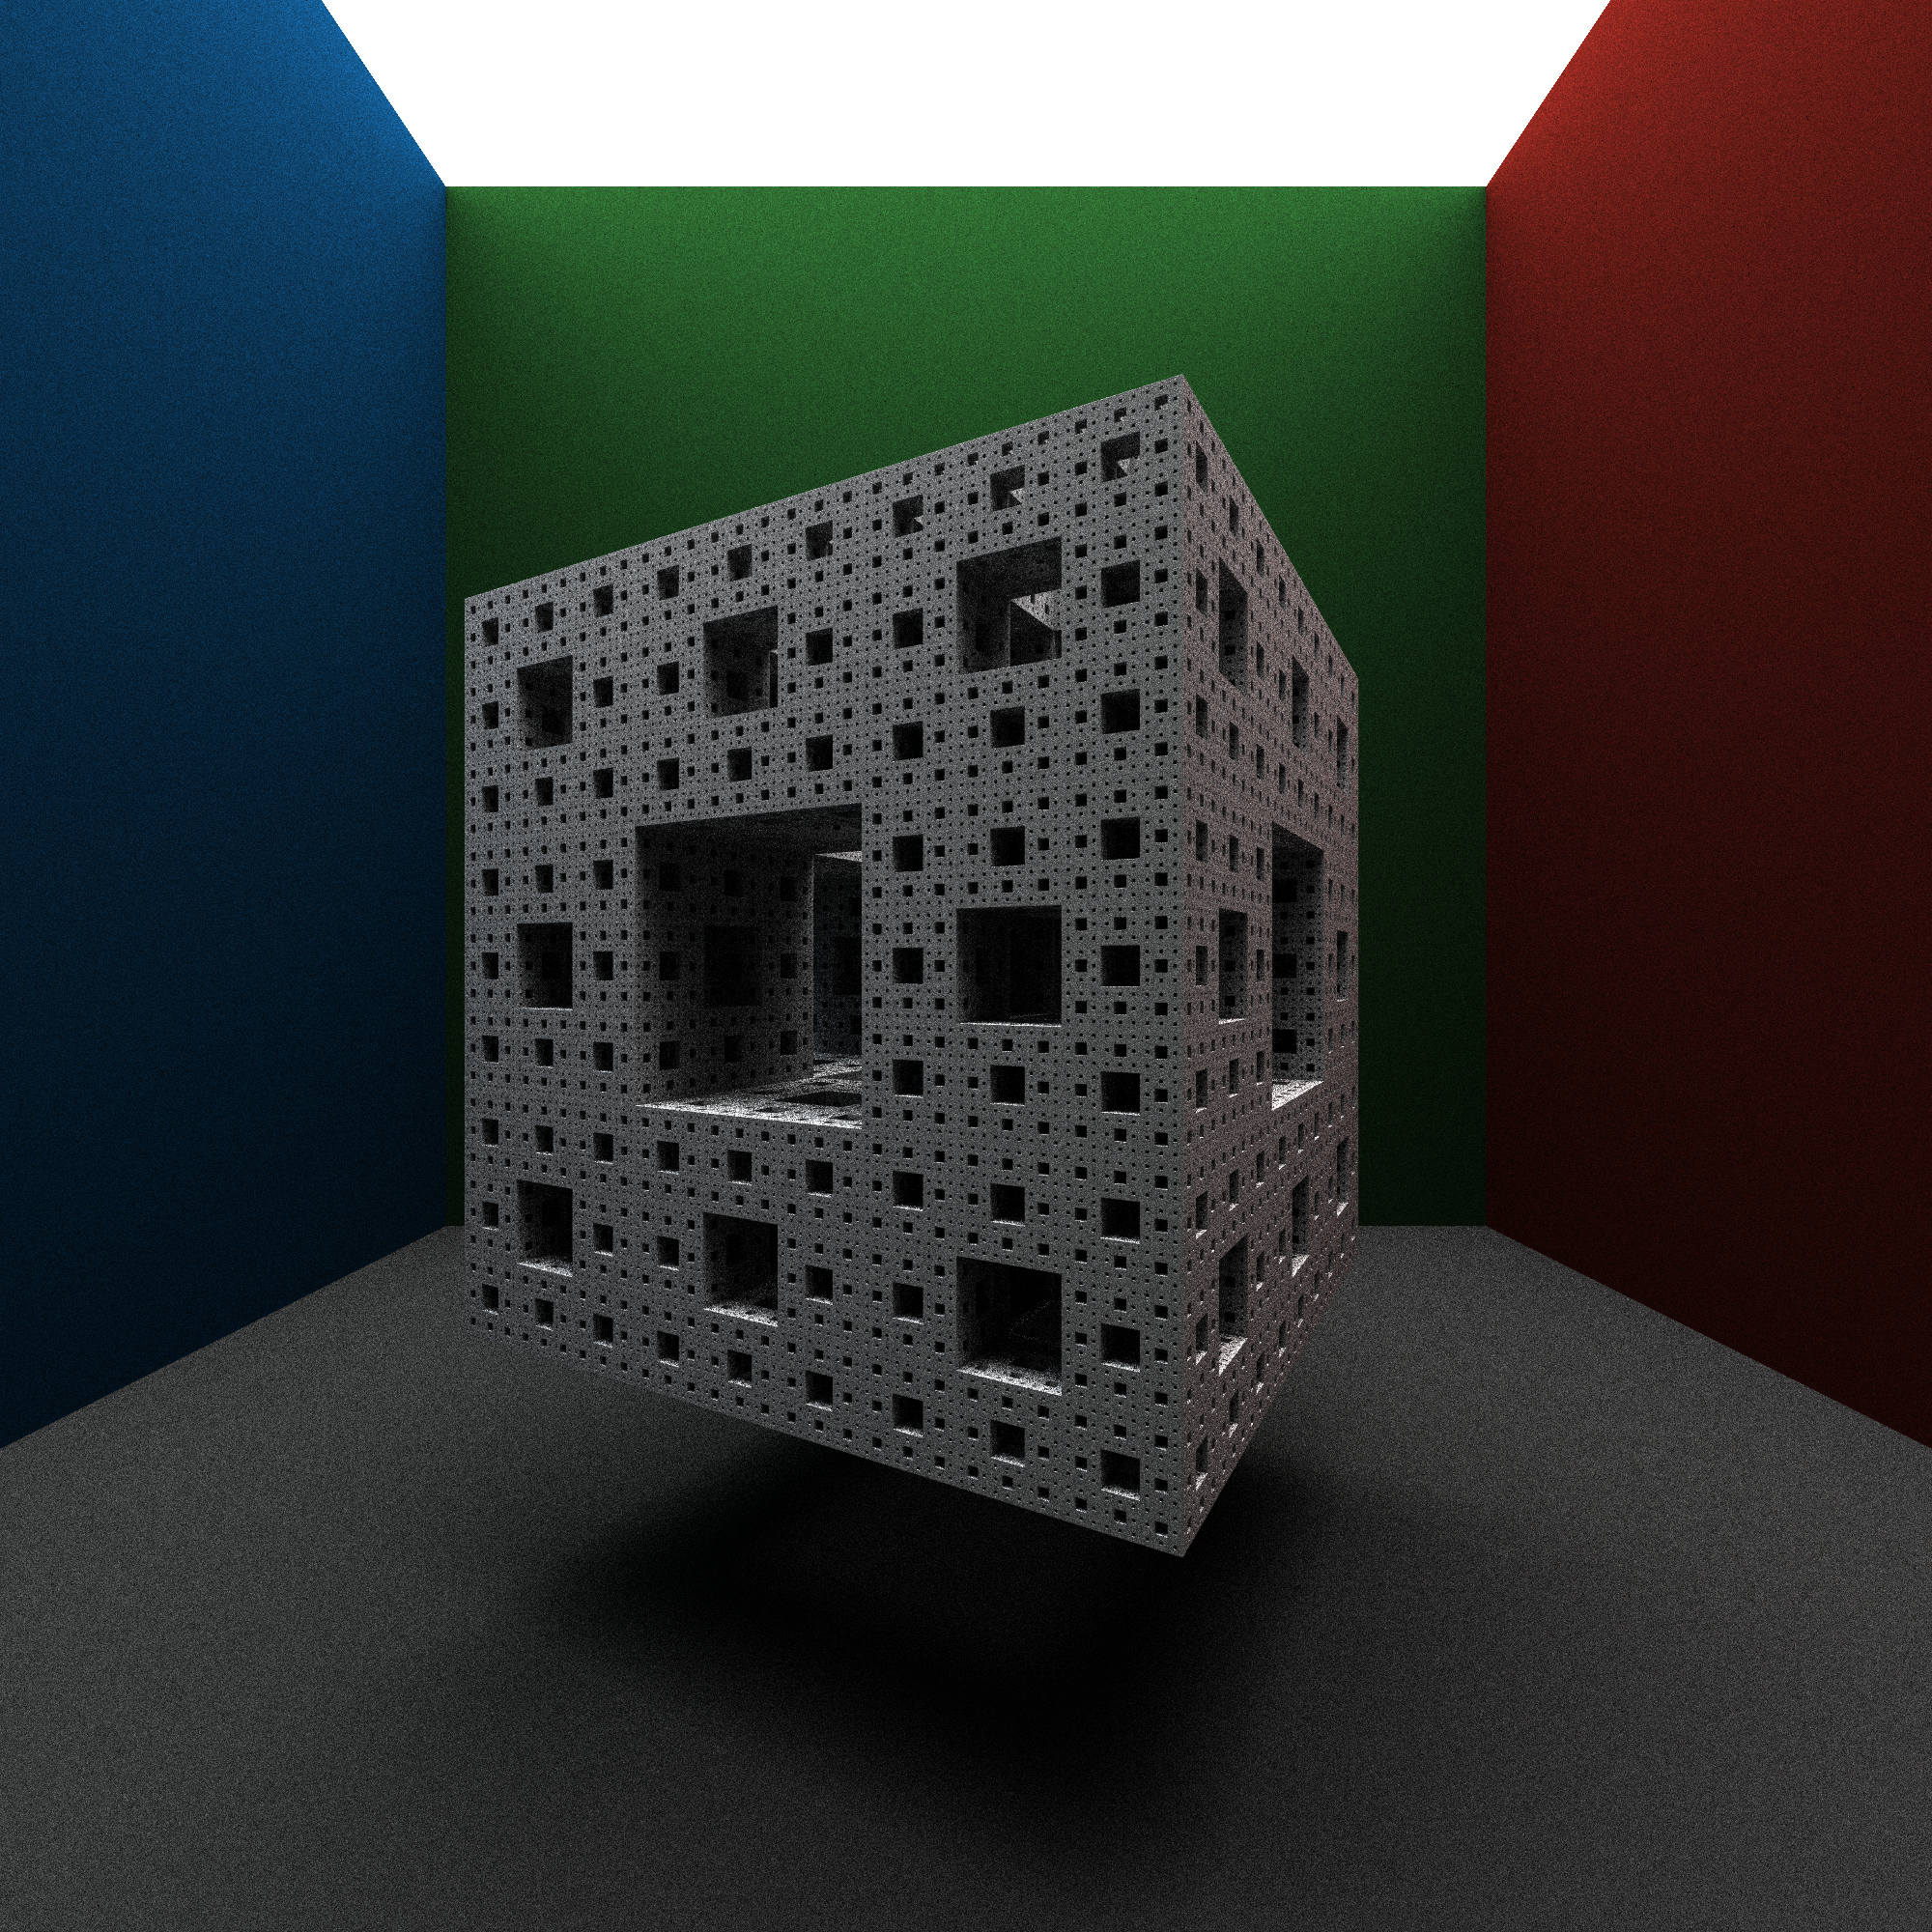
\includegraphics[width=\linewidth]{figures/menger.png}
    \caption{A more complex primitive of the menger sponge.}
  \endminipage\hfill
\end{figure}

\end{document}
